% !TeX root = ./ms.tex
\documentclass[modern]{aastex62}

% Shorthand
\newcommand{\STARRYQUADPOINTS}{100\xspace}
\newcommand{\kap}{\boldsymbol{\kappa}}
\newcommand{\kmt}{k^{-2}}
\newcommand{\vmax}{{v_\mathrm{max}}}

\newcommand{\DE}{\Delta \mathbf{E}(k^2, \kap)}
\newcommand{\DF}{\Delta \mathbf{F}(k^2, \kap)}

% Load the corTeX style definitions
% !TeX root = ./ms.tex
% All the packages
\usepackage{url}
\usepackage{amsmath}
\usepackage{mathtools}
\usepackage{amssymb}
\usepackage{natbib}
\usepackage{graphicx}
\usepackage{calc}
\usepackage{etoolbox}
\usepackage{xspace}
\usepackage[T1]{fontenc} % https://tex.stackexchange.com/a/166791
\usepackage{textcomp}
\usepackage{ifxetex}
\ifxetex
  \usepackage{fontspec}
  \defaultfontfeatures{Extension = .otf}
\fi
\usepackage{fontawesome}
\usepackage{listings}
\usepackage{nicefrac}
\usepackage[bb=boondox]{mathalfa}
\usepackage{booktabs}
\usepackage{longtable}

% Shorthand for this paper
\newcommand{\starry}{\textsf{starry}\xspace}
\newcommand{\Python}{\textsf{Python}\xspace}
\newcommand{\cpp}{\textsf{C}++\xspace}
\newcommand{\bvec}[1]{{\ensuremath{\mathbf{#1}}}}
\newcommand{\xxx}[1]{{\color{red}#1}}
\DeclarePairedDelimiter\floor{\lfloor}{\rfloor}
\DeclarePairedDelimiter\ceil{\lceil}{\rceil}
\newcommand{\imag}{{\ensuremath{\mathbb{i}}}}
\newcommand{\quadquad}{\quad\quad\quad\quad}

\newcommand{\R}{\bvec{R}}
\newcommand{\AOne}{\bvec{A_1}}
\newcommand{\alm}{\bvec{a}}
\newcommand{\x}{\bvec{x}}
\newcommand{\D}{D}
\newcommand{\Doppler}{\bvec{D}}
\newcommand{\Surf}{\mathcal{S}}
\newcommand{\Curve}{\mathcal{C}}
\newcommand{\Dargs}{\bvec{d}}
\newcommand{\lmax}{\ensuremath{l_\mathrm{max}}}
\newcommand{\spot}{\texttt{SPOT}\xspace}
\newcommand{\vogtstar}{\texttt{VOGTSTAR}\xspace}
\newcommand{\kT}{\boldsymbol{\kappa}^\top}
\newcommand{\rhoT}{\boldsymbol{\rho}^\top}
\newcommand{\ylmbasis}{\boldsymbol{\psi}^\top}
\newcommand{\pbasis}{\boldsymbol{\phi}^\top}
\newcommand{\pbasisn}{\ensuremath{\phi_n}}
\newcommand{\azero}{\ensuremath{\bvec{a_0}}}

% References to text content
\newcommand{\documentname}{\textsl{article}}
\newcommand{\figureref}[1]{\ref{fig:#1}}
\newcommand{\Figure}[1]{Figure~\figureref{#1}}
\newcommand{\figurelabel}[1]{\label{fig:#1}}
\renewcommand{\eqref}[1]{\ref{eq:#1}}
\newcommand{\Eq}[1]{Equation~(\eqref{#1})}
\newcommand{\eq}[1]{\Eq{#1}}
\newcommand{\eqalt}[1]{Equation~\eqref{#1}}

% Add code, proof, and animation hyperlinks
\definecolor{linkcolor}{rgb}{0.1216,0.4667,0.7059}
\newcommand{\codeicon}{{\color{linkcolor}\faFileCodeO}}
\newcommand{\prooficon}{{\color{linkcolor}\faPencilSquareO}}
\newcommand{\codelink}[1]{\href{https://github.com/user/repo/blob/fe12fa16a5cc76c1ba72d97241fb9545da144edf/tex/figures/#1.py}{\codeicon}\,\,}
\newcommand{\animlink}[1]{\href{https://github.com/user/repo/blob/fe12fa16a5cc76c1ba72d97241fb9545da144edf/tex/figures/#1.gif}{\animicon}\,\,}
\newcommand{\prooflink}[1]{\href{https://github.com/user/repo/blob/fe12fa16a5cc76c1ba72d97241fb9545da144edf/tex/proofs/#1.ipynb}{\raisebox{-0.1em}{\prooficon}}}
\newcommand{\cilink}[1]{\href{https://dev.azure.com/user/repo/_build}{#1}}


% Define a proof environment for open source equation proofs
\newtagform{eqtag}[]{(}{)}
\newcommand{\currentlabel}{None}
\newenvironment{proof}[1]{%
  \ifstrempty{#1}{%
    \renewtagform{eqtag}[]{\raisebox{-0.1em}{{\color{red}\faPencilSquareO}}\,(}{)}%
  }{%
    \renewtagform{eqtag}[]{\prooflink{#1}\,(}{)}%
  }%
  \usetagform{eqtag}%
  \renewcommand{\currentlabel}{#1}
  \align%
}{%
  \endalign%
  \renewtagform{eqtag}[]{(}{)}%
  \usetagform{eqtag}%
  \message{<<<\currentlabel: \theequation>>>}%
}

% Display the runtime on Azure
\usepackage[skins]{tcolorbox}
\newtcbox{\figtimebox}{enhanced,nobeforeafter,tcbox raise=-0.8mm,boxrule=0.6pt,
  top=0.5mm,bottom=0mm,right=0mm,left=6mm,arc=1pt,boxsep=2pt,
  before upper={\vphantom{dlg}},colframe=linkcolor,coltext=linkcolor,
  fontupper=\sffamily\bfseries\tiny,colback=white,overlay={\begin{tcbclipinterior}
        \fill[linkcolor] (frame.south west)
        rectangle node[text=white,font=\sffamily\bfseries\tiny,rotate=0]{CPU}
        ([xshift=6mm]frame.north west);\end{tcbclipinterior}}}
\robustify{\figtimebox}
\pdfstringdefDisableCommands{%
  \def\figtimebox#1{'#1'}%
}
\newcommand{\figtime}[1]{\IfFileExists{figures/#1.py.time}%
  {%
    \cilink{\figtimebox{\input{figures/#1.py.time}\unskip s}}
  }{}}

% Define the `oscaption` command for open source figure captions
\newcommand{\oscaption}[2]{\caption{#2 \codelink{#1} \figtime{#1}}}

% Code examples
\definecolor{codegreen}{rgb}{0,0.6,0}
\definecolor{codegray}{rgb}{0.5,0.5,0.5}
\definecolor{codepurple}{rgb}{0.58,0,0.82}
\definecolor{backcolour}{rgb}{0.95,0.95,0.95}
\lstdefinestyle{mystyle}{
  backgroundcolor=\color{backcolour},
  commentstyle=\color{codegreen},
  keywordstyle=\color{magenta},
  numberstyle=\tiny\color{codegray},
  stringstyle=\color{codepurple},
  basicstyle=\small\ttfamily,
  breakatwhitespace=false,
  breaklines=true,
  captionpos=b,
  keepspaces=true,
  numbers=left,
  numbersep=5pt,
  showspaces=false,
  showstringspaces=false,
  showtabs=false,
  tabsize=2,
  aboveskip=1em,
  belowskip=1em,
  keywords=[2]{map},
  keywordstyle=[2]{\color{black!80!black}},
  upquote=true
}
\lstset{style=mystyle}

% Typography obsessions
\setlength{\parindent}{3.0ex}
\renewcommand\quad{\hskip\fontdimen3\font}

% https://tex.stackexchange.com/a/184474
\usepackage{stackengine,scalerel}
\def\lnlam{\ThisStyle{\ensurestackMath{\stackon[-2.4\LMpt]{%
        \SavedStyle\lambda}{\kern-.5pt\kern\LMpt\rule{1\LMex}{.25pt+.15\LMpt}}}}}

% Bibliography stuff
\bibliographystyle{aasjournal}

% Begin!
\begin{document}

% Title
\title{Analytic Light Curves in Reflected Light}

% Author list
\author[0000-0002-0296-3826]{Rodrigo Luger}
\email{rluger@flatironinstitute.org}
\affil{Center~for~Computational~Astrophysics, Flatiron~Institute, New~York, NY}
%

\begin{abstract}
    Abstract here.
    %
    \href{https://github.com/rodluger/starrynight}{\color{linkcolor}\faGithub}
\end{abstract}

%
\section{Introduction}
%
This is an extension of \citep{Luger2019}.

%
\begin{figure}[h!]
    \begin{centering}
        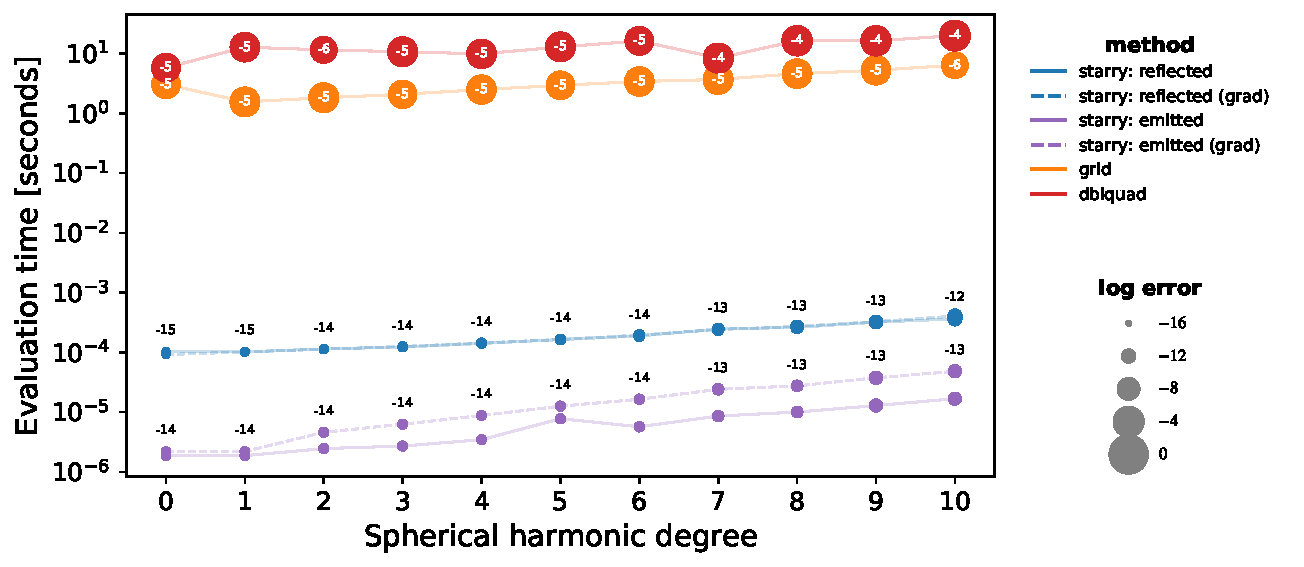
\includegraphics[width=\linewidth]{figures/speed.pdf}
        \oscaption{speed}{%
            Evaluation time for the starry algorithm.
            \label{fig:speed}
        }
    \end{centering}
\end{figure}

\section{Integration}

\subsection{Definitions}
%
Define the pairwise difference operator
%
\begin{align}
    \label{eq:pairdiff}
    \Delta \bvec{v} \equiv \sum_{i=0}^{\frac{N - 1}{2}}
    \left( v_{2i + 1} - v_{2i} \right)
\end{align}
%
which sums the difference of successive pairs of values in
an array $\bvec{v} = \{ v_0, v_1, v_2, v_3, {\cdot\cdot\cdot}, v_N\}$.

Define the quantity
%
\begin{align}
    \label{eq:q}
    \mathbf{q}(k^2, \kap) = \sqrt{1 - \frac{\sin^2\left(\frac{\kap}{2}\right)}{k^2}}
    \quad.
\end{align}

\subsection{$\mathcal{I}_v$}
%
The function $\mathcal{I}_v$ is given by
%
\begin{align}
    \label{eq:I}
    \mathcal{I}_v(k^2, \kap) =
    \sum_{i = 0}^{\frac{N - 1}{2}}
    \int\limits_{\frac{1}{2}\kappa_{2i}}^{\frac{1}{2}\kappa_{2i+1}}
    \sin^{2v}\varphi
    \mathrm{d}\varphi
    \quad.
\end{align}
%
The integral in this expression is the same as that in Equation (D38)
of \citet{Luger2019}, except for a change in the limits of integration.
As in \citet{Luger2019}, we can compute this integral recursively given
a trivial lower boundary condition:
%
\begin{proof}{I}
    \label{eq:Irec}
    \mathcal{I}_0(\kap) &=
    \frac{\Delta \kap}{2}
    %
    \nonumber \\
    %
    \mathcal{I}_v(\kap) &=
    \frac{1}{2v}
    \bigg(
    (2v - 1) \mathcal{I}_{v-1}(\kap) -
    \Delta \left(\sin^{2v - 1}\left(\frac{\kap}{2}\right)
    \cos\left(\frac{\kap}{2}\right)\right)
    \bigg)
\end{proof}
%
where the last expression is valid for all $v > 0$. We find that this algorithm
is generally stable, except when $\sin\left(\frac{\kap}{2}\right)$ is small. In
that limit, we evaluate $\mathcal{I}_N(\kap)$ by numerical integration of
Equation~(\ref{eq:I}) using Gauss-Legendre quadrature with \STARRYQUADPOINTS
points. We then recurse downward by substituting $v \rightarrow v + 1$ in
Equation~(\ref{eq:Irec}) and solving for $\mathcal{I}_v(\kap)$.

\subsection{$\mathcal{J}_v$}
%
The function $\mathcal{J}_v$ is given by
%
\begin{align}
    \label{eq:J}
    \mathcal{J}_v(k^2, \kap) =
    \sum_{i = 0}^{\frac{N - 1}{2}}
    \int\limits_{\frac{1}{2}\kappa_{2i}}^{\frac{1}{2}\kappa_{2i+1}}
    \sin^{2v}\varphi
    \left(1 - \frac{\sin^2\varphi}{k^2}\right)^\frac{3}{2}
    \mathrm{d}\varphi
    \quad.
\end{align}
%
The integral in this expression is again the same as that in Equation (D39)
of \citet{Luger2019}, except for a change in the limits of integration.
In that paper, we computed all terms
$\{ \mathcal{J}_0, {\cdot\cdot\cdot}, \mathcal{J}_\vmax \}$ from a three-term
recurrence relation and two boundary conditions. In the case of upward
recursion, the boundary conditions $\mathcal{J}_0$ and $\mathcal{J}_1$ were
computed analytically from the complete elliptic integrals $K(k^2)$
and $E(k^2)$. In cases where upward recursion was not numerically stable, we
evaluated $\mathcal{J}_\vmax$ and $\mathcal{J}_{\vmax-1}$
via a quickly convergent series expansion and recursed downward.

In order to solve Equation~(\ref{eq:J}), it is possible to
replace the complete elliptic integrals $K(k^2)$ and $E(k^2)$ in the lower
boundary conditions \citep[Equation D46 in ][]{Luger2019} with the
incomplete elliptic integrals $F(k^2, \kappa)$ and $E(k^2, \kappa)$,
then use the same upward
recursion relation to obtain analytic solutions for all $\mathcal{J}_v$:
%
\begin{proof}{J}
    \label{eq:Jrec}
    \mathcal{J}_0(k^2, \kap) &=
    \frac{1}{3} \bigg(
    2 \left(2 - \frac{1}{k^2}\right) \DE +
    \left(\frac{1}{k^2} - 1\right) \DF +
    \Delta \mathbf{z}_0(k^2, \kap)
    \bigg)
    %
    \nonumber \\
    %
    \mathcal{J}_1(k^2, \kap) &=
    \frac{1}{15} \bigg(
    \left(-3 k^2 + 13 - \frac{8}{k^2}\right) \DE +
    \left(3 k^2 - 7 + \frac{4}{k^2}\right) \DF +
    \Delta \mathbf{z}_1(k^2, \kap)
    \bigg)
    %
    \nonumber \\
    %
    \mathcal{J}_v(k^2, \kap) &=
    \frac{1}{2v + 3}
    \bigg(
    2 \left( v + 1 + (v - 1) k^2 \right) \mathcal{J}_{v - 1} -
    (2v - 3) k^2 \mathcal{J}_{v - 2}
    + \Delta \mathbf{z}_v(k^2, \kap)
    \bigg)
\end{proof}
%
%
where the last expression is valid for all $v > 1$ and
%
\begin{proof}{J}
    \label{eq:Jrec_z}
    \mathbf{z}_0(k^2, \boldsymbol{\kappa}) & =
    \frac{
        \sin\left(\frac{\kap}{2}\right)
        \cos\left(\frac{\kap}{2}\right)
        \mathbf{q}(k^2, \kap)
    }{
        k^2
    }
    %
    \nonumber                                  \\
    %
    \mathbf{z}_1(k^2, \boldsymbol{\kappa}) & =
    \left(\left(3 \sin^2 \left( \frac{\kap}{2} \right) + 4\right) - 6k^2\right)
    \mathbf{z}_0(k^2, \boldsymbol{\kappa})
    %
    \nonumber                                  \\
    %
    \mathbf{z}_v(k^2, \boldsymbol{\kappa}) & =
    k^2
    \sin^{2v - 3}\left( \frac{\kap}{2} \right)
    \cos\left( \frac{\kap}{2} \right)
    \mathbf{q}(k^2, \boldsymbol{\kappa})^5
    \quad.
\end{proof}
%
However, in practice we find that this procedure is even more numerically
unstable than it was in \citet{Luger2019}.
To address this, we express the recurrence structure of the problem as
a tridiagonal system with one lower boundary condition $\mathcal{J}_0$
and one upper boundary condition $\mathcal{J}_\vmax$:
%
\begin{proof}{J}
    \label{eq:Jtri}
    \begin{pmatrix}
        a_0 & 1   &     &        &         &         \\
        b_1 & a_1 & 1   &        &         &         \\
            & b_2 & a_2 & 1      &         &         \\
            &     & b_0 & a_3    & 1       &         \\
            &     &     & \ddots & \ddots  & \ddots  \\
            &     &     &        & b_\vmax & a_\vmax
    \end{pmatrix}
    \begin{pmatrix}
        \mathcal{J}_1   \\
        \mathcal{J}_2   \\
        \mathcal{J}_3   \\
        \mathcal{J}_4   \\
        \cdot\cdot\cdot \\
        \mathcal{J}_{\vmax-1}
    \end{pmatrix}
    =
    \begin{pmatrix}
        c_0 - b_0 \mathcal{J}_0 \\
        c_1                     \\
        c_2                     \\
        c_3                     \\
        \cdot\cdot\cdot         \\
        c_\vmax - \mathcal{J}_\vmax
    \end{pmatrix}
\end{proof}
%
where the recursion coefficients are given by
%
\begin{proof}{J}
    \label{eq:Jtri_coeffs}
    a_v(k) &= -2\frac{(v + 1) + (v - 1) k^2}{2v + 3} \nonumber \\
    b_v(k) &= \frac{(2v - 3) k^2}{2v + 3} \nonumber \\
    c_v(k^2, \kap) &= \Delta
    \bigg(
    \frac{
            \mathbf{z}_v(k^2, \boldsymbol{\kappa})
        }{
            2v + 3
        }
    \bigg)
    \quad.
\end{proof}
%
Solving this matrix system yields values for all
intermediate $\{ \mathcal{J}_1, {\cdot\cdot\cdot}, \mathcal{J}_{\vmax - 1} \}$.
While efficient algorithms exist for solving tridiagonal problems, we obtain
far better numerical stability by instead performing traditional LU
decomposition. We find that this algorithm is stable in all the regimes that we
tested.

We evaluate the upper boundary condition $\mathcal{J}_{\vmax}$ by numerical
integration of Equation~(\ref{eq:J}) via Gauss-Legendre quadrature with
\STARRYQUADPOINTS points. While the lower boundary condition may be computed
analytically from Equation~(\ref{eq:Jrec}),
in practice we achieve better precision via numerical
integration (as above), with negligible effects on computational performance.

\subsection{$\mathcal{W}_n$}
%
The function $\mathcal{W}_n$ is given by
%
\begin{align}
    \label{eq:W}
    % TODO
    \mathcal{W}_n = \int
\end{align}
%
This integral has a closed-form solution:
%
\begin{align}
    \label{eq:Wsol}
    \mathcal{W}_n =
    \frac{\sin^{2n + 2}\left(\frac{\kap}{2}\right)}{2n + 5}
    \left(
    \frac{3}{n+1}
        {_2F_1}\left(-\frac{1}{2}, n + 1; n + 2; 1 - q^2\right) + 2 q^3
    \right)
\end{align}
%
where ${_2F_1}(a, b; c; z)$ is the Gauss hypergeometric function.


% by either upward recursion (stable for |1 - q^2| > 1/2) or downward
% recursion (always stable).

% Bibliography
\bibliography{bib}


\end{document}
